\documentclass[a4paper,10pt]{article}
\usepackage[utf8]{inputenc}
\usepackage{amsmath}
\usepackage{amsfonts}
\usepackage{amssymb}
\usepackage{graphicx}
\usepackage{tikz}
\usepackage{amsthm}
%opening
\title{Parallel computation of the sequence of iterates of a function }
\author{Jean-Michel Fourneau \and Maël Guiraud \and Yann Strozecki}
\newcommand{\cS}{\mathcal{S}}
\newcommand{\todo}[1]{{\color{red} TODO: {#1}}}

 \newtheorem{theorem}{Theorem}
 
\begin{document}

\maketitle

\begin{abstract}

\end{abstract}

\section{Model}

Let $\cS$ be a finite set of states and let $f$ be a computable function from $\cS$ to $\cS$. 
The aim of this short article is to propose practical methods to compute the sequence $(s,f(s),\dots,f^n(s))$ in parallel.
When it is possible to compute efficiently $f^i(s)$ using only $s$ and $i$, it is easy to compute the sequence
in parallel by assigning one $f^i(s)$ to each processor. However, for general $f$ we need $f^{i}(s)$ to compute $f^{i+1}(s)$ and there is no simple scheme to parallelize the computation of the sequence. \todo{Is there a link with PPAD ?}
Hence, we consider additional structure on $\cS$ to make the problem tractable. The set $\cS$ is equipped with a partial order 
$\leq$ and it has a smallest element $\bot$ and a greatest element $ \top$. We assume that $f$ is monotone, that is 
if $s_1$ and $s_2$ are elements of $\cS$ such that $s_1 \leq s_2$ then $f(s_1) \leq f(s_2)$.


\todo{Define a simple model of parallelization + give a name to the problem}

This models a concrete problem: the simulation of a random process. In that setting, the function $f$ which describe the dynamic of the process also depends on the value of some random variable. In a simulation we use a random seed and then a random generator to generate the sequence of values of the random variable from the random seed. Say that the seed is a $m$ bit integers in $[2^m]$, we have a pseudo random generator $R$ which maps $[2^m]$ to $[2^m]$. A state of the system is $(s,y) \in \cS \times [2^m]$ where $s$ describes the state of the random process and $y$ is the current random number. A transition of the random process is given by a function $f$ from $\cS \times [2^m]$ to $\cS$ thus a pair $(s,x)$ is mapped to $(f(s,x),R(x))$ and we want to compute the iterates by this function.


\section{Method}

The main idea of the method is to divide $[n+1]$ into intervals of size $t$, on which the sequence of iterates will 
be computed independently.
We denote by $I_j$ the interval $\{tj, \dots, tj + t -1\}$. Each processor will be assigned the task to compute 
the sequence on some interval $I_j$ that is $(f^i(s))_{i \in I_j}$. We assume that we have some central memory in which the final solution is stored and to which each processor can write.


\subsection{Two bounds}

We describe an algorithm which produces the sequence  $(f^i(s))_{i\in [n+1]}$. Each interval $I_j$ has one of three states during the algorithm: $\textsc{ToCompute}$, $\textsc{InProgress}$ and $\textsc{Done}$ and we store for each interval $I_j$ the states $s_j^{min}$ and $s_j^{max}$.
The algorithm is the following: at the beginning, all intervals are marked $\textsc{ToCompute}$, for all $j >0$, 
$s_j^{min} = \bot$, $s_j^{max} = \top$ and $s_0^{min} = s_0^{max} = s$. 
In parallel, select a free processor $P$ and an interval $I_j$ in state $\textsc{ToCompute}$. 
The processor $P$ first and set the state of $I_j$ to $\textsc{InProgress}$ and then computes the two sequences $(f^i(s_j^{min}))_{i \in [t]}$ and $(f^i(s_j^{max}))_{i \in [t]}$ iteratively. When the sequences are computed, we have access to $f^t(s_j^{min})$ and 
 $f^t(s_j^{max})$. If $f^t(s_j^{min}) > s_{j+1}^{min}$ or $f^t(s_j^{max}) < s_{j+1}^{max}$ then better bounds have been found and $P$ sets $s_{j+1}^{min} = f^t(s_j^{min})$, $s_{j+1}^{max} = f^t(s_j^{max})$ and the state of $I_{j+1}$ to $\textsc{ToCompute}$.
Finally, if $s_j^{min}$ is equal to $s_j^{max}$, the result of the simulation is stored as the solution on the interval $I_j$
and $I_j$ is set to $\textsc{Done}$.

 \todo{écrire l'algo dans un environnement algo}
 
Remark that the choice of an interval with state $\textsc{ToCompute}$ by a free processor is not specified. 
In practice we propose two ways to select it. The first is to chose the interval of smallest index. 
The second is to cut $[n+1]$ into $l$ consecutive intervals (containing several $I_j$), where $l$ is the number of processors. 
Then we affect each processor to an interval and when it is free, we affect the smallest $I_j$ with state $\textsc{ToCompute}$ in this interval.  
 \todo{Etre bien plus précis dans les politiques de choix d'intervalle surtout pour le deuxième algo et lui donner un nom}
 
 \todo{Faire un petit modèle probabiliste qui pour une proba de coupler donnée combien on va faire de calculs.
 Ça serait bien de se servir de ça pour couper des intervalles de la bonne taille. }
 
 \begin{theorem}
  Algorithm TwoBounds produces the solution of the problem blah in a time 
  bounded by the one of the obvious sequential algorithm.
  \end{theorem}
  
\begin{proof}
We first prove that the algorithm terminates. At any point in time, there is a processor which is computing a part of the final solution. By induction on the time, assume a processor $P$ finishes to compute the sequence on an interval.
Then consider the smallest interval $I_j$ which is not marked $\textsc{Done}$. If it is in state $\textsc{InProgress}$, then 
 a processor is computing the solution on $I_j$. If it is in state $\textsc{ToCompute}$, it will be selected by the free processor $P$ and since $I_{j-1}$ is in state $\textsc{Done}$, $x_j^{min} = x_j^{max}$ and $P$ will compute the solution on $I_j$.

We must also prove that when an interval is set to $\textsc{Done}$, the right sequences of states has been computed. 
It follows from the fact that  $x_j^{min} \leq f^{jt}(s)$ and $x_j^{max} \geq f^{jt}(s)$. It can be proved by induction on the number of times the variables $x_j^{min}$ and  $x_j^{max}$ are updated, using the monotonicity of $f$ and the initialization of these variables to $\top$ and $\bot$. Hence when $x_j^{min} = x_j^{max}$ then it is also equal to $f^{jt}(s)$ and this value is enough to 
compute the sequence on $I_j$. 
\end{proof}

\todo{Donner une borne simple en moyenne quand les intervalles sont suffisemment long} 
 
Remark that all processors do the simulation using only their private memory and the two states at the beginning of the interval. This scheme is thus adapted to a distributed computing environment where the cost of transmitting information between processors is high. 


In our application to the simulation of a random process, the states of the process 
are often equipped with a partial order, but the random integers are not. 
However, we have the following property in our random system, if $s_1 \leq s_2$ then $f(s_1,x) \leq f(s_2,x)$. 
In fact, the random value alone is used to select an action to apply to the system and the action does not depends on the state of the system.

Since a random integer in the sequence depends only on the previous one, we can do the following trick to transform our problem.
Instead of using a single seed to generate all pseudo random values, use one seed for each interval $I_j$.
That is we have a collection of seeds $x_0, \dots x_{n/t}$ and the $i$th random number will be equal to 
$R^{i \mod t}(x_{i/t})$ instead of $R^i(x)$.
By doing that, we change the sequence we simulate, but it is still the same random process, that is all realizations
of the random process still occur with the same probability. 

\todo{Mieux expliquer cette partie}

\subsection{Algos avec intervalles de taille variables}

Inspiré de l'algo précédent mais plus souple. 
On coupe le temps en autant d'intervalles que de processeurs.
Ils sont simulés indépendemment et on note quand ça couple et on renvoie
la partie bien simulée, les seeds de la parties non couplée (seulement une petite partie). 
On réaffecte les processeurs sur les parties non encore trouvées


\subsection{One bound}


\section{Experiments}

The random process we use in our experiments is the following one. We have a system composed of $m$ finite queues of capacity BUFF\_MAX in tandem. A queue is characterized by its number of client $C_i$.  Every queue $i$ has tree events that can occurs:
\begin{itemize}
\item Arrival, $C_i$ is increased by one, if it is not already to BUFF\_MAX.
\item Service, a client leave the queue $i$ and goes in the queue $i+1$. $C_i$ is decreased by one and $C_{i+1}$ is increased by one. $C_{i+1}$ is equal to BUFF\_MAX, the client is lost.
\item Departure, the client leave the system. The number of client of the queue is decreased by one.
\end{itemize}

For the queue $i$, every event have a probability denoted by respectively $a_i$, $s_i$ and $d_i$. The last queue has no service, thus $s_m = 0 $. There is thus a total of $3m-1$ different events that can change the system.

The sequence that we want to parallelize is a succession of drawing of one of those $3m-1$ events. Every event is drawn randomly, following a pseudo random generator.

\begin{figure}
 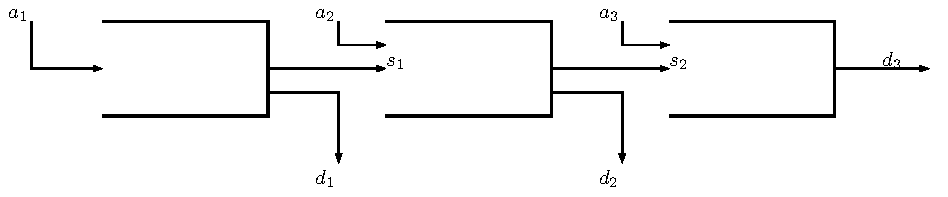
\includegraphics[scale=0.75]{figures/tandem.pdf}
 \caption{A system with 3 queues}
\end{figure}

\todo{ Precise description of the random process avec un dessin}

Our experimentations are made with the following set-up.
The program master is running on a MacBook Air, with a processor $2.2$ GHz Intel Core i$7$, and $8$ Go of RAM DDR$3$ at $1600$ MHz. The operating system of the machine is macOS High Sierra v$10.13.1$. The source code is compiled with  gcc version $7.1.0$ (Homebrew GCC $7.1.0$ --without-multilib).

We use up to $7$ servers are running on Raspberry Pi 3 , Model B, with $1GB$ of RAM. Their operating system is  Raspbian GNU/Linux $8.0$, installed on a micro SD card element$14$ with a size of $8$GB. The source code is compiled with gcc version $4.9.2$ (Raspbian $4.9.2-10$).

All the machines are connected on by a local network through an HP $14$-$10$ $8$G switch.

\todo{Description of the experimental settings: quel système d'exploitation/matériel/compilateur/librairies}

\todo{Experiments avec des jolies courbes et des interprétations}


Practical problems: cost of the network transmission, especially for transmitting long sequences.
-> measure the time of a two way trip for a small message and the time of sending an interval.
To say that in practice we will not compute the whole sequence but statistic on it which could help
reduce the use of the network.



\end{document}
